\documentclass[titlepage]{article}
\usepackage{graphicx} % Required for inserting images
\usepackage{fancyhdr}
\usepackage{tikz} 

\usepackage[hidelinks]{hyperref}
\hypersetup{
    linkcolor = blue,
}
\title{Computer Workshop \\ Final Assignment}
\author{Mohammad Amin Bahari}
\date{7 Bahman, 1402}
\pagestyle{fancy}
\fancyhead[L]{\thepage}



\begin{document}
\maketitle

\tableofcontents
\newpage
\section{Git and GitHub}

\subsection{Repository Initialization and Commits}
I created the repository from GitHub and added README.md file.
The i cloned the repo to my local computer and added main.tex file to the main directory.

\subsection{GitHub Actions for LaTeX Compilation}
from the action section i chose "set up a workflow yourself" and coppied the contents of main.yml from the example that was mentioned in the assignment.

\section{Exploration Tasks}

\subsection{Vim Advanced Features}
\begin{enumerate}
    \item Regular Expressions: Vim supports regular expressions for pattern matching and manipulation of text. Regular expressions (regex) allow you to search for and manipulate text based on patterns.
    \item Switch Case: it can switch case entire letters of a word with a command.
    \item Maros: they're a way to record and replay a list of commands.
\end{enumerate}

\subsection{Memory profiling}
\subsubsection{Memory Leak}
memory leaks happens when a program allocates memory but for some reason doesn't deallocate(frees) it. that leads to several issues in the program like slowing performance, behaving unexpectedly and more... .
\subsubsection{Memory profilers}
Valgrind is a programming tool for memory debugging, memory leak detection and profiling.
By scanning the program it detects everywhere that memory was dynamically allocated but never been deallocated and provides detailed info about memory leak.

\subsection{GNU/Linux Bash Scripting}
\subsubsection{fzf}
\begin{itemize}
    \item Fuzzy searching is a technique used in information retrieval to find approximate matches for a given search query, even when the query and the target data may not match exactly.
    \item The command ls | fzf is a combination of the ls command with the fzf utility to provide an interactive and visually appealing way to browse and select files from the current directory.
\end{itemize}

\subsubsection{ Using fzf to find your favorite PDF}
\texttt{fd -e pdf -t f -X -I | fzf}
type the name of your pdf and hit enter to select it.

\subsubsection{Opening the file using Zathura}
\texttt{zathura \$(fd -t d -e pdf -I | fzf)}




\section{Git and FOSS}
\subsection{README.md}
\subsection{Issues}
\begin{figure}
  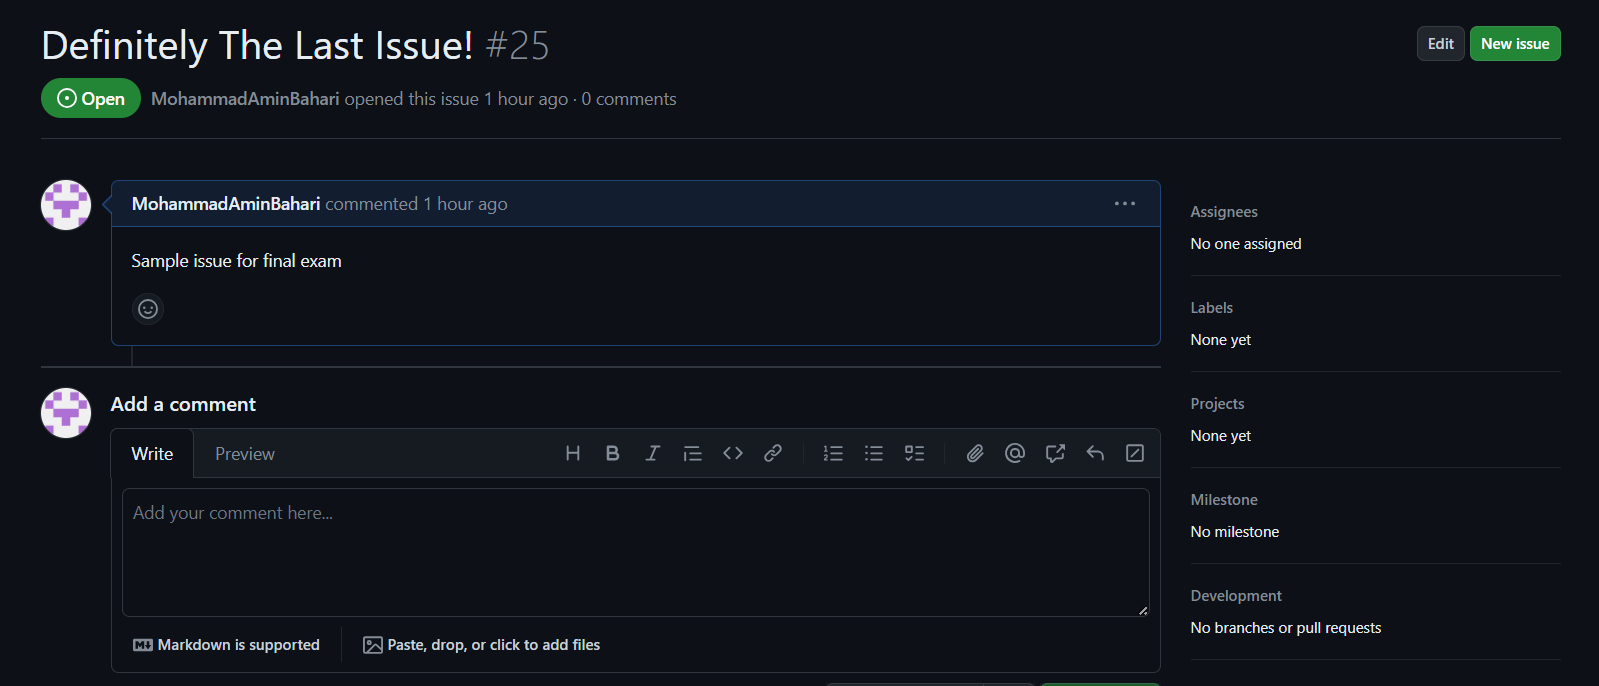
\includegraphics[width=\linewidth]{Capture.PNG}
  \caption{A boat.}
  \label{fig:boat1}
\end{figure}





\end{document}
